% This work is licensed under the Creative Commons
% Attribution-NonCommercial-ShareAlike 4.0 International License. To view a copy
% of this license, visit http://creativecommons.org/licenses/by-nc-sa/4.0/ or
% send a letter to Creative Commons, PO Box 1866, Mountain View, CA 94042, USA.

\section{Aufgabenblatt 7}

\subsection*{Aufgabe $\ast$)}
%TODO

\subsection*{Aufgabe $\ast\ast$)}
\textbf{Konvention:} $\cdot$ bindet stärker als $\cup$.

\subsection{Aufgabe 1}
Sei $\Sigma$ ein Alphabet und $X_1,X_2,Y_1,Y_2\subseteq\Sigma^\ast$ mit $X_1\subseteq Y_1$ und $X_2\subseteq Y_2$. Dann gilt:
\begin{enumerate}
	\item $X_1\cup X_2\subseteq Y_1\cup Y_2$, denn:\\
	Sei $x\in X_1\cup X_2$. 
	Dann ist $x\in X_1$ und somit $x\in Y_1$ und $x\in X_2\subseteq Y_2$. Folglich $x\in Y_1\cup Y_2$.
	\item $X_1\cdot X_2\subseteq Y_1\cdot Y_2$, denn:\\
	Sei $x\in X_1\cdot X_2$, d.h. es existiert $x_1\in X$, $x_2\in X_2$ so, dass $x=x_1\cdot x_2$. 
	Nach Voraussetzung gilt $x_1\in Y_1$ und $x_2\in Y_2$. 
	Folglich ist $x=x_1\cdot x_2\in Y_1\cdot Y_2$
	\item $X_1^\ast\cup Y_1^\ast$, denn:\\
	Sei $x\in X_1^\ast$. 
	Dann gibt es ein $n\in\N_0$ und $x_0,\ldots, x_n\in X_1$ mit $x=x_1\cdot\ldots\cdot x_n$. 
	Nach Voraussetzung gilt $x_1,\ldots,x_n\in Y_1$ und somit $x\in Y_1^\ast$.
\end{enumerate}

\subsection{Aufgabe 2}
Operatorpriorität: $\ast$ vor Exponent vor $\cdot$ vor $\cup,\cap$.

\subsubsection{Aufgabe 2 a)}
\begin{align*}
	&w\in L_1\cdot(L_2\cup L_3)\\
	&\Longleftrightarrow\exists u,v\in\Sigma^\ast:u\in L_1\wedge v\in L_2\cup L_3\wedge w=uv\\
	&\Longleftrightarrow\exists u,v\in\Sigma^\ast:u\in L_1\wedge \big(v\in L_2\vee v\in L_3\wedge w=uv\\
	&\Longleftrightarrow\exists u,v\in\Sigma^\ast:\big(u\in L_1\wedge v\in L_2\wedge v\in L_3\big)\vee\big(u\in L_1\wedge v\in L_3\wedge w=uv\big)\\
	&\Longleftrightarrow\Big(\exists u,v\in\Sigma^\ast:u\in L_1\wedge v\in L_2\wedge v\in L_3\Big)\vee
	\Big(\exists u,v\in\Sigma^\ast:u\in L_1\wedge v\in L_3\wedge w=uv\Big)\\
	&\Longleftrightarrow w\in L_1\cdot L_2\vee w\in L_1\cdot L_3\\
	&\Longleftrightarrow w\in L_1\cdot L_2\cup L_1\cdot L_3
\end{align*}

\subsubsection{Aufgabe 2 b)}
Die Aussagen gilt.

\begin{proof}
	Zeige zuerst mit natürlicher Induktion, dass für alle $n\in\N$ gilt:
	\begin{align*}
		\lbrace ab,a\rbrace^n\cdot\lbrace a\rbrace=\lbrace a\rbrace\cdot\lbrace ba,a\rbrace^n
	\end{align*}
	\ul{IA}: $n=0$: $\lbrace ab,a\rbrace^0\cdot\lbrace a\rbrace=\lbrace\varepsilon\rbrace\cdot\lbrace a\rbrace=\lbrace\varepsilon\cdot a\rbrace=\lbrace a\rbrace=\lbrace a\cdot\varepsilon\rbrace=\lbrace a\rbrace\cdot\lbrace\varepsilon\rbrace=\lbrace a\rbrace\cdot\lbrace ba,a\rbrace^0$\nl
	\ul{IH}: Für $n\in\N$ gilt $\lbrace ab,a\rbrace^n\cdot \lbrace a\rbrace=\lbrace a\rbrace\cdot\lbrace ba,a\rbrace^n$\nl
	\ul{IS:}
	\begin{align*}
		\lbrace ab,a\rbrace^{n+1}\cdot\lbrace a\rbrace
		&=\lbrace ab,a\rbrace^{n}\cdot\lbrace ab,a\rbrace\cdot\lbrace a\rbrace\\
		&=\lbrace ab,a\rbrace^{n}\cdot\lbrace aba,aa\rbrace\\
		&=\lbrace ab,a\rbrace^{n}\cdot\lbrace a\rbrace\cdot \lbrace ba,a\rbrace\\
		\overset{\text{IV}}&=
		\lbrace a\rbrace\cdot\lbrace ba,a\rbrace^n\cdot\lbrace ba,a\rbrace\\
		&=\lbrace a\rbrace\cdot\lbrace ba,a\rbrace^{n+1}
	\end{align*}
	Damit kann nun die ursprüngliche Aussage gezeigt werden:
	\begin{align*}
		w\in\big(\lbrace a\rbrace\cdot\lbrace b\rbrace\cup\lbrace a\rbrace\big)^\ast\cdot\lbrace a\rbrace\\
		&\Longleftrightarrow
		w\in \lbrace ab,a\rbrace^\ast\cdot\lbrace a\rbrace\\
		&\Longleftrightarrow
		\exists k\in\N_0:w\in\lbrace ab,a\rbrace^k\cdot\lbrace a\rbrace\\
		\overset{\text{Indu}}&\Longleftrightarrow
		\exists k\in\N_0:w\in\lbrace a\rbrace\cdot\lbrace ba,a\rbrace^k\\
		&\Longleftrightarrow
		w\in\lbrace a\rbrace\cdot\lbrace ba,a\rbrace^\ast\\
		&\Longleftrightarrow
		w\in\lbrace a\rbrace\cdot\big(\lbrace b\rbrace\cdot\lbrace a\rbrace\cup\lbrace a\rbrace\big)^\ast
	\end{align*}
\end{proof}

\subsubsection{Aufgabe 2 c)}
Falsch, betrachte folgendes Gegenbeispiel:\\
$a\in\big(\lbrace a\rbrace\cup\lbrace b\rbrace\big)\ast=\lbrace a,b\rbrace^\ast$, aber $ab\not\in\lbrace^\ast\cup\lbrace b\rbrace^\ast=\lbrace\varepsilon, a,aa,aaa,\ldots,b,bb,bbb,\ldots\rbrace$

\subsubsection{Aufgabe 2 d)}
Für alle $L\subseteq\Sigma^\ast$ gilt $L^0:=\lbrace\varepsilon\rbrace$ und $L\cdot\emptyset=\emptyset\cdot L=\emptyset$. Daher gilt:
\begin{align*}
	\emptyset^\ast=\bigcup\limits_{n\geq0}\emptyset^n=\emptyset^0\cup\emptyset^1\cup\emptyset^2\cup\ldots=\lbrace\varepsilon\rbrace\cup\emptyset\cup\emptyset\cup\ldots=\lbrace\varepsilon\rbrace
\end{align*}
Offensichtlich gilt: $L\cup L\cup\lbrace\varepsilon\rbrace$. 
Damit folgt mit der Monotonie (Aufgabe 1):
\begin{align*}
	\big(\cup\lbrace\varepsilon\rbrace\big)^\ast\supseteq L^\ast
\end{align*}
Sei nun $w\in \big(L\cup\lbrace\varepsilon\rbrace\big)^\ast$. 
Dann existiert $k\in\N$ mit $w\in\big(L\cup\lbrace\varepsilon\rbrace\big)^k$. 
Zeige nun per Induktion über $n\in\N$: $w\in\big(L\cup\lbrace\varepsilon\rbrace\big)^n\implies L^\ast$.\nl
\ul{IA}: $n=0$: $\big(L\cup\lbrace\varepsilon\rbrace\big)^0=\lbrace\varepsilon\rbrace=L^0\subseteq L^\ast$\nl
\ul{IH:} Für $n\in\N$ gelte: $w\in\big(L\cup\lbrace\varepsilon\rbrace\big)^n\implies w\in L^\ast$\nl
\ul{IS:} Sei $w\in\big(L\cup\lbrace\varepsilon\rbrace\big)^{n+1}=\big(L\cup\lbrace\varepsilon\rbrace\big)^n\cdot\big(L\cup\lbrace\varepsilon\rbrace\big)$. Dann existiert $u\in\big(L\cup\lbrace\varepsilon\rbrace\big)^n$ und $v\in\big(L\cup\lbrace\varepsilon\rbrace\big)$ mit $w=uv$.\\
\begin{itemize}
	\item $v=\varepsilon$: Dann $w=u$. Aus IH folgt dann $w\in L^\ast$.
	\item $v\in L\setminus\lbrace\varepsilon\rbrace$: Aus IH $u\in L^\ast$, d.h. es existiert $m\in\N$ mit $u\in L^m$. 
	Dann gilt $w=u\cdot v\in L^m\cdot L=L^{m+1}$ und damit auch $w\in L^\ast$
\end{itemize}

\subsubsection{Aufgabe 2 e)}
Gilt.

\subsubsection{Aufgabe 2 f)}
Gilt.

\subsection{Aufgabe 3}
Idee: Füge Zustände ein, so, dass an den Pfeilen Worte von höchstens Länge 1 sind.

\usetikzlibrary{positioning,automata}
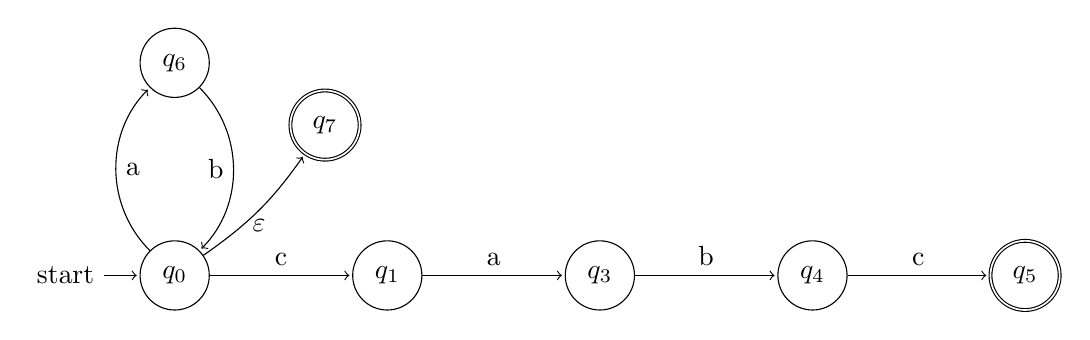
\begin{tikzpicture}[shorten >=1pt,node distance=2.7cm,on grid]
  \node[state,initial]   (q_0)                {$q_0$};
  \node[state]           (q_1) [right=of q_0] {$q_1$};
  \node[state]           (q_2) [right=of q_1] {$q_3$};
  \node[state]           (q_3) [right=of q_2] {$q_4$};
  \node[state,accepting] (q_4) [right=of q_3] {$q_5$};
  \node[state]           (q_5) [above=of q_0] {$q_6$};
  \node[state,accepting] (q_6) [above right=of q_0] {$q_7$};
  \path[->] (q_0) edge                node [above] {c} (q_1)
                  edge [bend left=45] node [right] {a} (q_5)
                  edge [bend right=10]node [below] {$\varepsilon$} (q_6)
            (q_1) edge                node [above] {a} (q_2)
            (q_2) edge                node [above] {b} (q_3)
            (q_3) edge                node [above] {c} (q_4)
            (q_5) edge [bend left=45] node [left] {b} (q_0);
\end{tikzpicture}

\subsection{Aufgabe 4}
Ziel: $\varepsilon$-Kanten entfernen: Dazu Anpassung von Übergangsrelation und Endzuständen:
\begin{align*}
	\Delta'&:=\left\lbrace(p,a,q)\in Q\times\Sigma\times Q:p\stackrel{a}{\longrightarrow}_\mathcal{A} q\right\rbrace\\
	F'&:=\left\lbrace\begin{array}{cl}
		F\cup\lbrace q_0\rbrace, &\falls q_0\stackrel{\varepsilon}{\longrightarrow}_\mathcal{A} a\mit q\in F\\
		F, &\sonst
	\end{array}\right.
\end{align*}

\usetikzlibrary{positioning,automata}
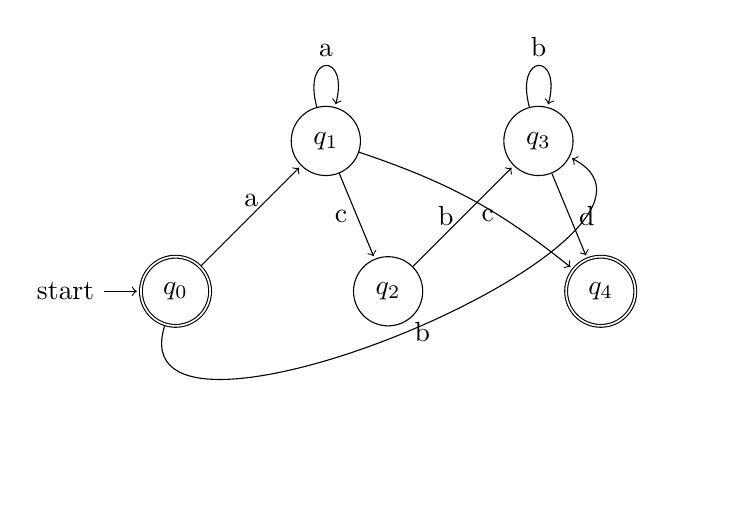
\begin{tikzpicture}[shorten >=1pt,node distance=2.7cm,on grid]
  \node[state,initial,accepting](q_0)               {$q_0$};
  \node[state]           (q_1) [above right=of q_0] {$q_1$};
  \node[state]           (q_2) [right=of q_0]       {$q_2$};
  \node[state]           (q_3) [above right=of q_2] {$q_3$};
  \node[state,accepting] (q_4) [right=of q_2]       {$q_4$};
  \path[->] (q_0) edge                node [above] {a} (q_1)
                  edge [bend left=230] node [right] {b} (q_3)
            (q_1) edge [loop above]   node [above] {a} ()
            	  edge                node [left]  {c} (q_2)
            	  edge [bend left=10] node [below right] {c} (q_4)
            (q_2) edge                node [left] {b} (q_3)
            (q_3) edge                node [right] {d} (q_4)
            	  edge [loop above]   node [above] {b} ();
\end{tikzpicture}

\subsection{Aufgabe 5}
Transitionssystem ist NEA mit potenziell mehreren Anfangszuständen und potenziell unendlich viele Zustände akzeptiert

\subsubsection{Aufgabe 5 a)}
\usetikzlibrary{positioning,automata}
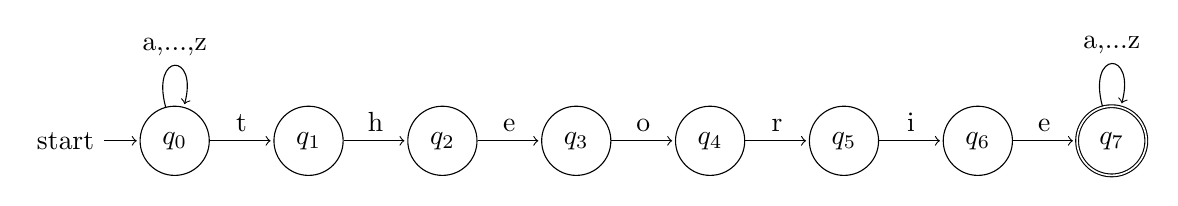
\begin{tikzpicture}[shorten >=1pt,node distance=1.7cm,on grid]
  \node[state,initial]   (q_0)                {$q_0$};
  \node[state]           (q_1) [right=of q_0] {$q_1$};
  \node[state]           (q_2) [right=of q_1] {$q_2$};
  \node[state]           (q_3) [right=of q_2] {$q_3$};
  \node[state]           (q_4) [right=of q_3] {$q_4$};
  \node[state]           (q_5) [right=of q_4] {$q_5$};
  \node[state]           (q_6) [right=of q_5] {$q_6$};
  \node[state,accepting] (q_7) [right=of q_6] {$q_7$};
  \path[->] (q_0) edge [loop above]   node [above] {a,...,z} ()
                  edge                node [above] {t} (q_1)
            (q_1) edge                node [above] {h} (q_2)
            (q_2) edge                node [above] {e} (q_3)
            (q_3) edge                node [above] {o} (q_4)
            (q_4) edge                node [above] {r} (q_5)
            (q_5) edge                node [above] {i} (q_6)
            (q_6) edge                node [above] {e} (q_7)
            (q_7) edge [loop above]   node [above] {a,...z} ();
\end{tikzpicture}

\subsubsection{Aufgabe 5 b)}
Für $\Sigma=\lbrace a\rbrace$:\\
\usetikzlibrary{positioning,automata}
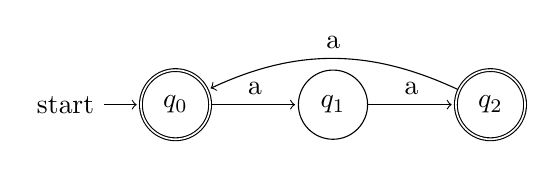
\begin{tikzpicture}[shorten >=1pt,node distance=2cm,on grid]
  \node[state,initial,accepting]   (q_0)                {$q_0$};
  \node[state]           (q_1) [right=of q_0] {$q_1$};
  \node[state,accepting] (q_2) [right=of q_1] {$q_2$};
  \path[->] (q_0) edge              node [above] {a} (q_1)
  			(q_1) edge              node [above] {a} (q_2)
  			(q_2) edge [bend right =25] node [above] {a} (q_0);
\end{tikzpicture}

Für $\Sigma=\lbrace a,b\rbrace$:\\
\usetikzlibrary{positioning,automata}
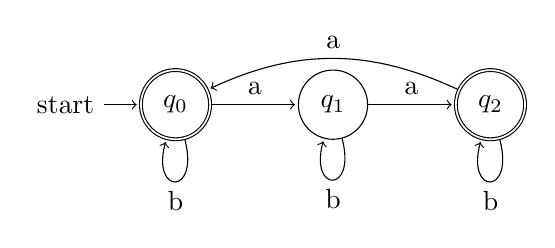
\begin{tikzpicture}[shorten >=1pt,node distance=2cm,on grid]
  \node[state,initial,accepting]   (q_0)                {$q_0$};
  \node[state]           (q_1) [right=of q_0] {$q_1$};
  \node[state,accepting] (q_2) [right=of q_1] {$q_2$};
  \path[->] (q_0) edge              node [above] {a} (q_1)
  				  edge [loop below] node [below] {b} ()
  			(q_1) edge              node [above] {a} (q_2)
  			      edge [loop below] node [below] {b} ()
  			(q_2) edge [bend right =25] node [above] {a} (q_0)
  			      edge [loop below] node [below] {b} ();
\end{tikzpicture}

\begin{align*}
	Q_1 &=\big\lbrace q_0,q_1,q_2\big\rbrace,\qquad I_1=\lbrace q_0\rbrace,\qquad F_1=\lbrace q_0\rbrace\\
	\Delta_1&=\big\lbrace(q_0,a,q_1),(q_1,a,q_2),(q_2,a,q_0)\big\rbrace
\end{align*}
Beachte: Das Tikz-Bild beschreibt genau die Definition von $\Delta_1$.
\subsection*{Aufgabe 5 c)}
%TODO Tikz Bild
\subsection*{Aufgabe 5 d)}
%TODO Tikz Bild
